\documentclass[oneside]{book}

\setcounter{tocdepth}{1}
\setcounter{secnumdepth}{3}

\usepackage[toc,page]{appendix}
\usepackage{hyperref}
\usepackage[utf8]{inputenc}
\usepackage{graphicx} % Required for the inclusion of images
\usepackage{amsmath} % Required for some math elements 
\usepackage[utf8]{inputenc}
\usepackage[english]{babel}
\newtheorem{theorem}{Theorem}
\newtheorem{corollary}{Corollary}[theorem]
\newtheorem{lemma}[theorem]{Lemma}
\usepackage{listings}
\usepackage{pdfpages}
\usepackage{amssymb}
\usepackage{pdflscape}

\begin{document}

\begin{titlepage}
	\centering
	
\includegraphics[width=0.60\textwidth]{../../logo/UoN_Primary_Logo_RGB.png}\par\vspace{1cm}
	\vspace{1.5cm}
	{\huge\bfseries Replicating the Sugarscape Model in FrABS \par}
	\vspace{2cm}
	{\Large\itshape jonathan.thaler@nottingham.ac.uk \par}
	\vfill
	
	\vfill

	{\large \today\par}
\end{titlepage}

\cleardoublepage

\section*{Abstract}
This report describes the work and results done to replicate the Sugarscape Model as presented in the book "Growing Artificial Societies - Social Sciences from the bottom up" by Joshua M. Epstein and Robert Axtell \cite{epstein_growing_1996}.

\clearpage
\tableofcontents
\clearpage

\section{Introduction}
There exists a large number of simulation packages which allow the convenient creation of System Dynamics simulations by straight-forward visual diagram creation. One simply creates stocks and flows, connects them, specifies the flow-rates and initial parameters and then runs the model. An example for such a visual diagram creation in the simulation package AnyLogic can be seen in Figure \ref{fig:sir_stockflow_diagram}.

\begin{figure}
	\centering
	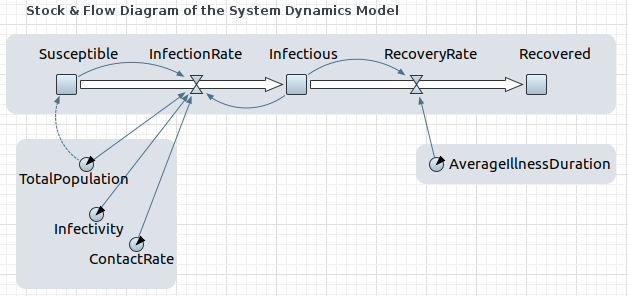
\includegraphics[width=.5\textwidth, angle=0]{./fig/SIR_SD_STOCKFLOW_DIAGRAMM.png}
	\caption{Visual System Dynamics Diagram of the SIR model in AnyLogic Personal Learning Edition 8.3.1.}
	\label{fig:sir_stockflow_diagram}
\end{figure}

Still, implementing System Dynamics directly in code is not as straight forward and involves numerical integration which can be quite tricky to get right. Thus, the aim of this paper is to look into how System Dynamics models can be implemented in code correctly without the use of a simulation package. We use the well known SIR model \cite{kermack_contribution_1927} from epidemiology to demonstrate our approach.

Our language of choice is Haskell because it emphasises a declarative programming style in which one describes \textit{what} instead of \textit{how} to compute. Further it allows to rule out interference with non-deterministic influences or side-effects already at compile-time. This is of fundamental importance for System Dynamics because it behaves completely deterministic and involves no stochastics or non-determinism whatsoever. Also, we make use of Functional Reactive Programming which allows to express continuous-time systems in a functional way. 

We show that by this approach we can arrive at correct-by-construction implementations of System Dynamic models. This means that the correctness of the code is obvious because we have closed the gap between the model specification and its implementation. Thus, the contribution of the paper is the demonstration of how to implement correct-by-construction System Dynamics simulations using Haskell and Functional Reactive Programming.

\section{Chapter II: Life And Death On The Sugarscape}

\section{Chapter III: Sex, Culture, And Conflict: The Emergence Of History}



%\section{Chapter IV: Sugar and Spice - Trade Comes to the Sugarscape}
TODO: the most complex chapter, not done so far. The time for this will be when starting to look into correctness of ABS in the second half of the 2nd year (somewhere around february 2018)

%\section{Chapter V: Disease Processes}
TODO: although it is not the most complex chapter, we also haven't replicated it so far. The time for this will be when starting to look into correctness of ABS in the second half of the 2nd year (somewhere around february 2018)

\renewcommand\bibname{References}

\bibliographystyle{acm}
\bibliography{../../references/phdReferences}

\end{document}
